\chapter{Математические модели синтеза топологии сети для охвата линейного участка в виде задачи целлочисленного линейного программирования}

Эффективным способом повышения технико-экономических показателей при проектировании \fixme{БШС} является оптимизация топологии сети, а именно решение задачи выбора оптимального набора станций из заданного избыточного множества и определение мест их размещения вдоль линейной контролируемой территории.
Основным результатом работы, представленной в этой главе, является разработка итерационного метода выбора оптимальной топологии сети в процессе комплексного проектирования БШС. 
Принципиальной особенностью предлагаемого метода, повышающей его эффективность, является то, что для рассмотрения на этапе моделирования предлагается не одно решения, а последовательности лучших решений задачи оптимизации топологии сети. Это позволяет с помощью разработанной итерационной процедуры выбирать на этапе моделирования лучшее решение среди тех решений по топологии, которые удовлетворяют требуемым характеристикам проектируемой БШС. 

\section{Постановка задачи и ее формулировка в экстремальной комбинаторной форме}

\section{Introduction}
At the present time, the problem to supervise and control the area where industrial and civil facilities, technological installations, moving vehicles, etc. , are placed, is a very important. 

	The problem of optimal equipment placement on a given redundant set of possible placement locations comes to light in the process of creating the distributed control systems. In this paper we consider the infrastructure consisting of multiple base stations that interact to each other to form the broadband communication network.
 	
 	We review the particular case of a such problem, when the territory to be controlled is a one-dimensional linear route. It could be a section of a road transportation network, a linear part of a main pipeline, or a field communications line. For example, a backbone network of road side units (RSUs) is an essential part of modern intelligent transportation systems, where the roadside units are used to collect and distribute information among the mobile users.
 	
%  \begin{figure}
% \includegraphics[width=\textwidth]{fig1.eps}
% \caption{Optimal station placement problem parameters including places and stations description.} \label{fig1}
% \end{figure}
 	Similar problems were discussed in a number of publications. Brahim et. al. ~\cite{ref1} describes the problem of station deployment which will maximize the coverage area while restricted by a total cost. The input data includes the set of potential places for stations deployment and the preliminarily collected statistics of the users’ traffic. Cavalcante et. al. suggested the model of maximum coverage with delay restrictions and analyzed it with the genetic algorithm ~\cite{ref2}. The problem of correct choice of road side units placement scheme for maximizing coverage of territory are presented in ~\cite{ref3}. Liu et. al. ~\cite{ref4} formulated road side units (RSUs) placement problem which will maximize the probability of the average connectivity in vehicular ad-hoc network as a combinatorial optimization problem. The problem is solved by the Expansion and Coloration Algorithm (ECA), with an addition of taking into consideration the road traffic characteristics. In articles ~\cite{ref5,ref6} the authors consider the extremal problem of choosing base station types and their placement along the line road. They formulated and discussed the problem in a form of the mixed - integer programming model.
	
	Within the framework of a wide class of optimal placement of capacities problems, the problem considered in this article in addition to the specificity of one-dimensional structure of the territory to be controlled, also has the substantial feature caused by distance limit presence between base stations. 
	
	The main result of our work is the development of a special branch and bound algorithm for solving the problem of optimal location for the given set of base stations in wireless network with linear topology represented in a combinatorial form. The paper also describes  the problem statement in the form of a mixed – integer linear programming model. The results of a comparative computational experiments to solve the problem: (a) by the brute force method, (b) by the branch and bound method and (c) in the form of the mixed - integer linear programming model  are presented. 
	
\section{The placement problem in the combinatorial form}

Let be we have a line segment $\alpha$ of length $L$ with the ends points $a_0$ and $a_{n+1}$. Inside of the segment $\alpha = [a_0, a_{n+1}]$ a finite set of arranged points $A = \{a_i\}_{i=1}^n, \, a_{i+1} > a_i$ is given; these points correspond to the set of vacant places where the stations can be placed. Each point $a_i$ is defined with its one-dimensional coordinate $l_i$. Let's also denote a set of stations as $S = \{s_j\}_{j=1}^m$. Each station has two parameters: a coverage radius $r_j$ and a communication radius $R_j$. Then we can also define a station $s_j\in S$ as a set of parameters: $s_j = \{r_j, R_j\}$.

There are special stations $s_0$ and $s_{n+1}$ which are gateways. These stations are already placed at the ends $a_0$ and $a_{n+1}$ of the segment 
$\alpha$ correspondingly. For those stations  $r_0 = r_{n+1} = 0$ and $R_0 = R_{m+1} = 0$. 

A \textit{feasible stations placement} $P = \{a_i, s_j\}$ is a sequence of pairs for which the following constraints are satisfied:

\begin{enumerate}
	\item left connectivity: $\forall\;(a_i, s_j),\,1 \leq i \leq n,$ either $\exists (a_k, s_q):\:l_k < l_i $ 
	and $l_i - l_k \leq \min \{R_j, R_q \},$ or $l_i - l_0 \leq R_j$;
	\item right connectivity: $\forall\;(a_i, s_j),\,1 \leq i \leq n,$ either $\exists (a_t, s_g):\:l_t > l_i $ 
	and $ l_t - l_i \leq \min \{R_j, R_g \}, $ or $ l_{n+1} - l_i \leq R_j$;	
	\item $|P| = m$.
\end{enumerate}

The first and the second requirements guarantee that all stations are connected in a chain and this chain ends in the gateways. The third requirement guarantee that all stations have been placed. 

Let’s define the set of all feasible placements as $G$. 

The coverage value $z(P)$ is corresponded to each placement $P$.  This function is defined as the length of disjoint union 
of segments $\tau,\tau \subset \alpha$ such that each segment is included in the coverage only if it is contained in the coverage 
area of some station from placement $P$, and each point $a \in \alpha$ belongs to a single segment $\tau$.

We introduce the concept of "non-coverage" of the segment $\alpha$:

\begin{displaymath}
f(P) = L - z(P)
\end{displaymath} 

Now we can formulate the optimal placement problem as the extremal combinatorial problem in the combinatorial form.

\textit{Problem 1.}

It is required to find a permissible placement $P^*$, such that
\begin{displaymath}
P^* = \argmin \limits_{P \in G} f(P)
\end{displaymath}

Let us denote the set of all combination of $m$ stations on $n$ places (not only feasible placements) as $\Gamma$. The number of elements $\gamma \in \Gamma$ is

\begin{displaymath}
\gamma = C_n^m \times m!
\end{displaymath} 


\section{The brute-force method}

To solve the problem described above, we will first consider the brute-force method. For it to be implemented we define an algorithm to build a binary search tree, also referred to as a branch tree. This algorithm will be also useful for us to develop the branch and bound algorithm that will be described further.

The algorithm builds a tree by splitting a set $G$. This approach involves a use of a well - known method based on a variation of a binary variable. The variable $\pi_{ij}$ that is used for splitting is defined as follows:


\begin{itemize}
	\item $\pi_{ij} = 1$ if the station $s_j$ is placed into point $a_i$;
	\item $\pi_{ij} = 0$ otherwise.
\end{itemize}

The procedure is an iterative one: on $\nu$ iteration we fix the value of the variable $\pi_{ij}$ to 0 or 1 that will cause the splitting the entire set $G_\nu$ into two child subsets $G^1_\nu$  and $G^2_\nu$, which correspond to child vertexes of the parent vertex corresponding to the set $G_\nu$ on the branch tree. Let’s assume that $G^1_\nu$ is obtained by setting $\pi_{ij} = 1$ and $G^2_\nu$  is obtained by setting $\pi_{ij} = 0$.

Now we will describe how we choose such variable among the set of all variables $\Pi = \{\pi_{ij}\}$. Based on previously chosen variables and its values on some iteration, the given set forms a disjoint union of three sets: $\Pi^+$ – the set of variable equals to 1 (allowed variable), $\Pi^-$ – the set of variables equals to 0 (forbidden variable), and $\Pi^f$ – undefined variables.

To split the set $G_\nu$ the variable $\pi_{ij}$ are chosen among $\Pi^f$ with the lowest possible $i$ and $j$. It means that we decide: either locate the station $s_j$  on the place $a_i$ or not.

We describe movement on the branch tree.

After splitting the set $G_\nu$ in two subsets $G_\nu^1$  and $G_\nu^2$, these subsets on the branch tree are assigned the indices $G_{\nu+1}$  and$G_{\nu+2}$, respectively.

When forming a branch tree, two types of steps are defined: the “direct” step and the “back” step. The direct step is the movement “in depth” along the same branch of the tree to execute  the  partition of the current subset $G_\nu$. The back step is the step which performs the transition from the set $G_\nu$ to one of the previously formed subsets. The back step is executed in cases when either the set $G_\nu$  consists of one variant of  station location or the set $G_\nu$ is empty. In these cases, the corresponding vertex of the tree is called “closed”.

For movement on a tree we will use the LIFO rule. Direct steps will be performed until a vertex is obtained that must be closed. This corresponds to a movement along the same tree branch. The subset $G_\nu^1$ will be examine first of the subsets $G_\nu^1$  and $G_\nu^2$.

If the vertex will be not be closed as a result of the examination, then further movement on the same branch will continue (the execution of a direct step). If the vertex will be closed, then the back step will be executed. The back step is the transferred to the unclosed vertex which is the last formed vertex among unexamined vertexes.

The process stops after set of  $\Pi^f$ becomes empty.

\section{The branch and bound algorithm}\label{sec:proof}
We have developed the branches and bound algorithm to reduce the search on the branch tree.

In order to develop the branch and bound algorithm for solving the placement problem using the branch tree described in the previous section, we need only to develop methods for investigating vertices for the possibility of closure.  
  
In accordance with the branch and bound technique the vertex will be closed in following three cases. 

\textit{Case 1.} Set $G_\nu$ is empty, i.e. there is no feasible placement for given sets of allowed and forbidden variables.

\textit{Case 2.} It has been proved that in set $G_\nu$ there is no feasible placement with the value of objective function $f(P)$ which is less than already found $f(\widehat{P})$ named as "current best value". The initial value of $f(\widehat{P})$ is set higher then possible optimal value (e.g.  $f(\widehat{P})$ is L).

\textit{Case 3.} An optimal solution for set $G_\nu$ has been found.

\subsection{Case 1.}
Here we should proof that conductivity or completeness constraints described above are not fulfilled.

To prove completeness infeasibility, it is sufficient to show that for given allowed and forbidden $\pi_{ij}$ there is no vacant place for some unplaced station.  

Obviously, such a check is algorithmically easy to implement: it suffices to show that there exists $k$ such that for a station $s_{k}$ for which $\pi_{ik} \neq 1$ for all $i$ there is no $a_i$ for which simultaneously $\pi_{ij}
 \neq 1$  for some $j$, $j \neq k$, and $\pi_{ik} \neq 0$.

To prove connectivity infeasibility, we first should check the following requirement for the initial set $G = G_0$: the distance between two neighboring places should not be greater than the second largest communication radius $R_j$. of stations in $S$. If the requirement is not satisfied, then the set of all feasible placements G is empty and the problem has not the solution.

We will describe now the check procedure for $G_\nu$, $\nu$ > 0. We will assume that $G_\nu$ is obtained by splitting the parent set by variable $\pi_{kt}$ = 1 and the set contains more than one placement $P$. The algorithm consists of three steps.

\textit {Step 1.} Check that each distance $R_t$ and $R_h$, where $h$ is an index of a station placed into position $a_d$ just before $a_k$, is greater than $l_k$ - $l_d$. If the closest place from the left is $a_0$ than it checks $R_t$ only.

\textit {Step 2.} Check that both $R_t$ and the largest $R_j$ between unplaced stations is not less than the distance between $a_k$ and place $a_i$, the closest to it from the right. If such place is $a_{n+1}$ the check is applied only to $R_t$ and the distance $l_{n+1}$ - $l_k$.
If all stations are placed, then $G_\nu$ consists of the single placement and this case will be analyzed further.

\textit {Step 3.} If the number of unplaced stations is more than 1, then we check that the distance between the two neighboring points is not greater than the second largest communication radius among unplaced stations, and the distance between $a_{n+1}$ and $a_{n}$ is not greater than the largest one. 

If only one unallocated station remains, then we check that among the still unoccupied points to the right of the point $a_k$  there is at least one such point that the distances from this point to the point $a_k$ and simultaneously from this point to the point $a_{n+1}$ is no greater than the communication radius $R_j$ of the station remaining unallocated.

If on at least one step is failed, then $G_\nu$ is empty and the vertex must be closed. In this case, the back step is performed.

If the set $G_\nu$ is obtained by setting $\pi_{kt}$ = 0, then one should check that the distance between the place with the greatest index among those where stations are placed (considering $a_0$) and $a_k$ is not exceeded the maximum connectivity range of unplaced stations.  If this is not true, then the set $G_\nu$  is empty and the back step is performed.

\subsection{Case 2.}
Let us name as a \textit {partial non – coverage} the value

\begin{equation}\label{eq1}
\Delta(k,d,p,t) = max\{\left(a_{k} - a_{d} \right) - \left(r_{p} - r_{t} \right), 0\}.
\end{equation}

This value is defined for any two places $a_d$ and $a_k$, $k > d$, where the stations $s_p$ and $s_t$ are placed in situations  where  there is no other station between them.

It is obvious that non – coverage $f(P)$ for every placement $P$ is calculated as the sum of all $\Delta(k,d,p,t)$ between the places where stations are deployed including the ends of $\alpha$.

Let us build the lower bound $W(G_\nu)$ for $f(P)$, i. e.

\begin{displaymath}
W(G_\nu) \leq f(P), P \in G_\nu. 
\end{displaymath}

If it can be shown that $W(G_\nu) \geq f(\widehat{P})$, then $G_\nu$ does not contain the placement better than already found $\widehat{P}$ and the vertex should be closed.
 
First we shall build $W(G_0)$.

Since all the stations must be placed, then the maximum coverage of $\alpha$ is obtained in situations when  it would be possible to place all the stations without intersections of their coverage radiuses . Each station $s_j$ covers the segment of length 2$r_j$, therefore, a total non - coverage cannot exceed the value.

\begin{displaymath}
W\left(G_0\right) = \max{\left\{L-\sum_{j=1}^{m}{2r_j,0}\right\}}.                                                                                  
\end{displaymath}

Now we will define $W(G_\nu)$, $\nu > 0$ as the sum of partial sums $w_1$ and $w_2$. 

\begin{displaymath}
W\left(G_\nu\right) = w_1 + w_2.                                                                                  
\end{displaymath}

Suppose $G_\nu$ is obtained by splitting a parent set by setting the variable $\pi_{kt}$ = 1. Then $w_1$ is "non-coverage" of the segment from $a_0$ to $a_k$ while $w_2$ is non-coverage of the segment from $a_k$ to $a_{n+1}$.

The sum $w_1$ is calculated by formula (\ref{eq1}) by summing non-coverages between the places where stations have been placed already. 

The sum $w_2$ is calculated as

\begin{equation}\label{eq2}
w_2 = max\left\{\left(l_{n+1}-l_k\right)-\left(r_t+\sum_{j\in S_v}{2r_j}\right),0\right\},
\end{equation}
where $S_\nu$ is the set of unplaced stations. 

The formula (\ref{eq2}) is analogous to the formula (\ref{eq1}) except the fact, that it is applicable to the part of segment $\alpha$ which is to the right from the last place where any station has been placed.

If $\pi_{kt}$ = 0 the estimation $W(G_{\nu})$ remains unchanged after splitting.

\subsection{Case 3.}
In this case we review only sets $G_\nu$, which consist of a single placement $P$, and $f(P)$ is obtained as the sum of non-coverages $\Delta(k,d,p,t)$ between known places where  stations are placed.

 If for the given placement the inequality $f(P) < f(\widehat{P})$ takes place, then the placement $P$ becomes a new current best value $\widehat{P}$ and backward step is applied.
 
The branch and bound algorithm will stop when all the vertexes of the searching tree will be closed.
 
The solution is
\begin{displaymath}
P^{*} = \widehat{P},  \widehat{f}(P^*) = f(\widehat{P}).
\end{displaymath}

\section{Example 1}

\textit{Input data.}

The segment $\alpha$  with $L$ = 50, end points $a_0$  and  $a_4$  with coordinates $l_0$ = 0 and $l_4$= 50 is given. There are internal  points $a_1$, $a_2$, $a_3$ with coordinates $l_1$ = 20, $l_2$= 30, $l_3$=40.

The set of stations $S=\left\{s_j\right\}, j=1,2$  is given, where station $s_j$ has parameters: $r_1$ = 20, $R_1$ = 40; $r_2$ = 5, $R_2$ = 20. There are special stations $s_0$ and $s_4$, on the end points with $r_0$=$R_0$= 
$r_4$=$R_4$=0.

We have to find a feasible placement $P^*$, such that

\begin{displaymath}
P^* = \min \limits_{P \in G} f(P)
\end{displaymath}

The process of solving the problem is presented in the form of a binary search tree (see Fig.~\ref{fig2}).
 
The initial value of $f(\widehat{P})=L=50$, $G_0=G$.

The vertices of the tree indicated by $\emptyset$  correspond to the sets $G_\nu$ for which there are no feasible placements.

Two placements $P_1$ and $P_2$ were obtained as the current best solutions  with $f(P_1)=15$ and $f(P_2)=5$.

The optimal solution is $P^\ast=P_2,\ \ f\left(P^\ast\right)=f\left(P_2\right)=5$.

\begin{figure}
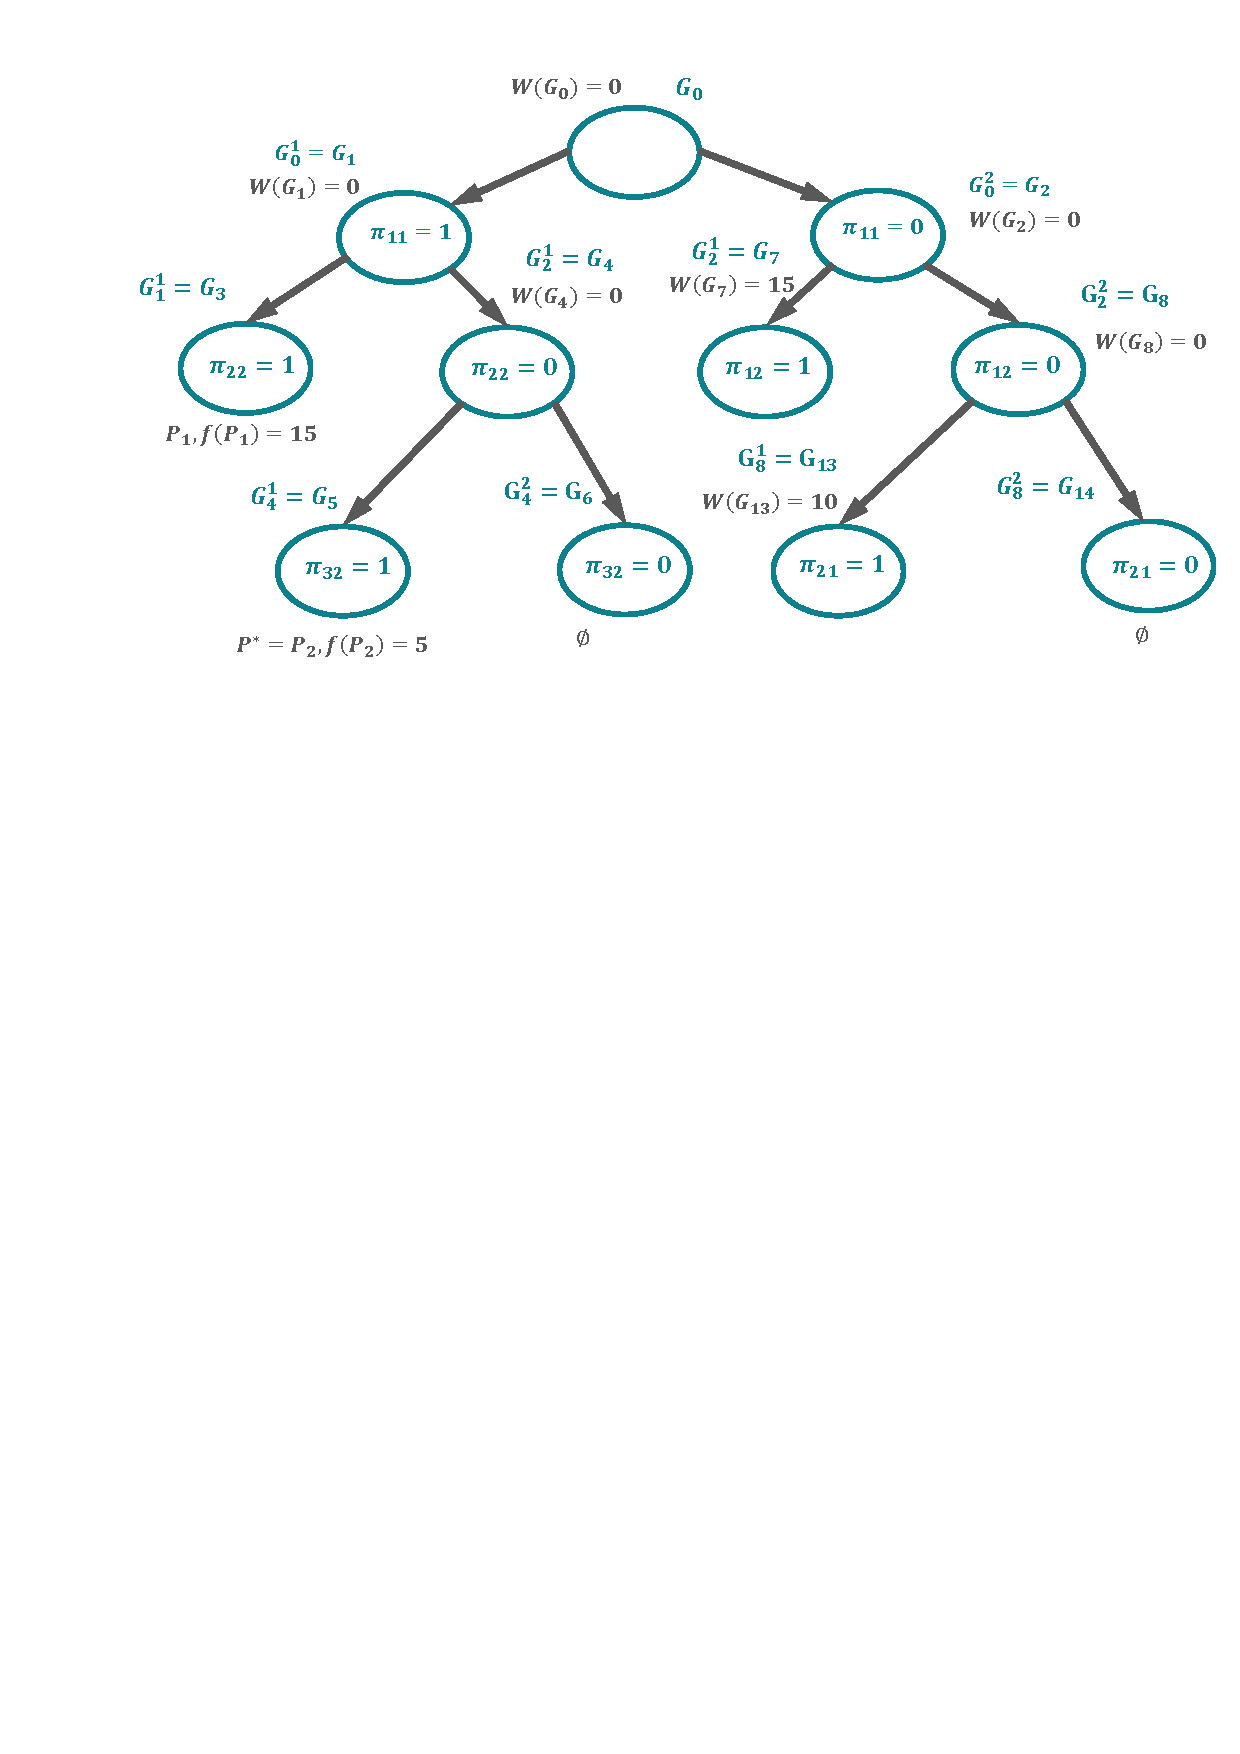
\includegraphics[width=\textwidth]{tree.pdf}
\caption{The search tree of branch and bound algorithm.} \label{fig2}
\end{figure}

\section{The statement of problem as a mixed – integer programming model}
Here we will formulate our placement problem in the form of a mixed – integer programming model. The description of problem is given in section 2.

Let us introduce binary variables $x_{ij}$ where $x_{ij}=1$ if a station $s_j$ is placed at point $a_i$ and $x_{ij}=0$ otherwise.

Let us introduce binary variables $e_i$ where $e_i$=1 if any station is placed at point $a_i$ and $e_i=0$ otherwise.

By definition

\begin{displaymath}
e_i=\sum_{j}^{m}{x_{ij}}, i=1,2,\ldots,n.
\end{displaymath}

We have $e_0$ = 1 and $e_{n+1}$ = 1 for the end points.

Let us formulate the following system of the problem constraints.

Each station must be placed in one and only one place

\begin{displaymath}
\sum_{i=1}^{n}{x_{ij}=1}, j=1,2,\ldots,m.
\end{displaymath}

At any point there can be no more than one station

\begin{displaymath}
\sum_{j=1}^{m}{x_{ij} \leq 1}, i=1,2,\ldots,m.
\end{displaymath}

We will introduce non-negative variables $y_i^+$  and  $y_i^-$ for points $a_i$, $i=0,1,2,..,n$, $n+1$.
Variables $y_i^+$ and  $y_i^-$  are the area sizes (right and left from point $a_i$) which are covered by station placed at point $a_i$.

Values of  variables $y_0^+$, $y_0^-$,$y_{n+1}^+$, $y_{n+1}^-$ equal 0.

The values of coverages are not greater than the coverage radius of the station located at $a_i$, and equal to 0 if is no station at $a_i$:

\begin{displaymath}
y_i^+\le\sum_{j=1}^{m}{x_{ij}r_j} ,i=1,2,\ldots,n,
\end{displaymath}

\begin{displaymath}
y_i^-\le\sum_{j=1}^{m}{x_{ij}r_j} ,i=1,2,\ldots,n.
\end{displaymath}

The total coverage area between any two points $a_i$ and $a_k$ on which the stations are located cannot exceed the distance between these points.

For  $i=1,\ldots,n$:

\begin{displaymath}
y_i^+ + y_k^- \le\frac{l_k - l_i}{2}\left(e_i + e_k\right)+\left(2 - e_i - e_k\right)L, k=i+1,\ldots,n+1,
\end{displaymath}

\begin{displaymath}
y_i^- + y_k^+  \le\frac{l_i - l_k}{2}\left(e_i + e_k\right)+\left(2 - e_i - e_k\right)L ,k=i-1,\ldots,0.
\end{displaymath}

	This condition excludes the effect from intersections of station coverages when calculating the total coverage value for the entire segment $\alpha$.
	
	According to the conditions of the problem, the station located at $a_i$ must be connected with at least one station on the left and one station on the right, including stations  at the end points $a_0$ and $a_{n+1}$.

	We will introduce variables $z_{ijk}, i=1,2,\ldots,n$; $j=1,2,\ldots,m$; $k=1,2,\ldots,n$; $k\neq i$ to formulate this requirement where:

\begin{itemize}
	\item $z_{ijk}=1$ if a station $s_j$ is located at point $a_i$ and connected with a station which is located at point  $a_k$;
	\item $z_{ijk}=0$ otherwise.
\end{itemize}	
	
	We will also introduce variables $z_{ij0}$ and $z_{ijn+1}$ where $z_{ij0}=1$ if a station $s_j$ is located at point $a_i$ and connected with a station $s_0$ which is located at point  $a_0$  and $z_{ij0} = 0$ otherwise; $z_{ijn+1}=1$ if a station $s_j$ is located at point $a_i$ and connected with a station $s_{n+1}$ which is located at point $a_{n+1}$  and $z_{ijn+1} = 0$ otherwise.

Stations must be at both points so that they can be connected: 

\begin{displaymath}
z_{ijk}\le e_i,  \forall i,j,k,
\end{displaymath}

\begin{displaymath}
z_{ijk}\le e_k, \forall i,j,k.
\end{displaymath}

The station $s_j$ which is located at $a_i$ must be connected with at least one station which is located right from $a_i$ and at least one station  which is located left from $a_i$

\begin{displaymath}
\sum_{k=i+1}^{n+1}{z_{ijk} \geq x_{ij}}, \forall i,j,
\end{displaymath}

\begin{displaymath}
\sum_{k=0}^{i-1}{z_{ijk} \geq x_{ij}}, \forall i,j.
\end{displaymath}

The communication radius $R_j$ of the station located at the point  $a_i$, must be no less than the distance to the point $a_k$, where there is a station with which it is connected:

\begin{displaymath}
z_{ijk\ }\left(R_j-\left(a_i-a_k\right)\right)\geq 0, k=i-1,\ldots,0, j=1,2,\ldots,m,  
\end{displaymath}

\begin{displaymath}
z_{ijk}\left(R_j-\left(a_k-a_i\right)\right)\geq 0, k=i+1,\ldots,n+1, j=1,2,\ldots,m. 
\end{displaymath}

Objective function

\begin{displaymath}
f=\sum_{i=1}^{n}{\left(y_i^++y_i^-\right)\rightarrow max} 
\end{displaymath}


\section{Numerical results}
The algorithms Branch and Bound (BnB) and brute-force algorithm (BF) were implemented using Python.
Table 1 shows the results of solving several problems for a different number of locations and a different number of stations using the B and B algorithm, the BF algorithm and the standard program for solving mixed – integer problem in the MATLAB package. We compare the number of vertices in the search trees so that the execution parameters of the algorithms do not depend on the speed of the machine and/or the quality the computer program. For each set of stations and set of placements   10 examples were computed with different numerical input data. For B and B and the MATLAB package the table shows the average execution parameters of the number of vertices in the search tree for each of the 10 examples.

\begin{table}
\caption{The results of solving problems.}\label{tab1}
\begin{tabular}{|l|l|l|l|l|}
\hline
{\bfseries Places} & {\bfseries Stations} &	{\bfseries BF}& {\bfseries BnB} & {\bfseries MILP} \\ 
\hline
7 &		5 &	17550  &	933 &		753\\
9 &		5 &	71090  &	6478 &		2669\\
10 &	5 &	126180 &	1041 &		8551\\
12 &	6 &	No &		8294 &		38569\\
13 & 	6 &	No &		18485 &		30369\\
\hline
\end{tabular}
\end{table}

\textit {The numerical results. “No” means the problem was not solved after 3 hours}. 

\section{Conclusion}

In this  paper the problem of finding optimal location for the  given set of base stations in wireless network with linear topology was analyzed. The problem has been formulated as an  extremal combinatorial problem and also as mixed – integer linear programming model.  The branch and bound algorithm for solving the problem in combinatorial form was developed. The results of the computer experiment show that the branch and bound algorithm is more effective than the brute-force algorithm and using of the branch and bound algorithm also more effective than to solve the problem represented as a mixed–integer programming model.
